% Wissenswertes:
% \todo und \missingfigure erzeugen eine Warning: bad box, Underfill ... -> diese kann ignoriert werden

\documentclass[fontsize=12pt, a4paper, headinclude, twoside=false, parskip=half+, pagesize=auto, numbers=noenddot, plainheadsepline, open=right, toc=listof, toc=bibliography, chapteratlists=0pt]{scrreprt}

% Allgemeines
\usepackage{scrlayer-scrpage} % Kopf- und Fußzeilen
\usepackage{amsmath,marvosym} % Mathesachen
\usepackage[T1]{fontenc} % Ligaturen, richtige Umlaute im PDF
\usepackage[utf8]{inputenc}% UTF8-Kodierung für Umlaute usw
\usepackage{caption}
\usepackage[Q=yes]{examplep}
\usepackage[colorinlistoftodos, textwidth=\marginparwidth]{todonotes}
\let\oldmissingfigure\missingfigure % save old command
\renewcommand{\missingfigure}[1]{\oldmissingfigure[figwidth=\textwidth-2pt]{#1}}% renew \missingfigure command
\usepackage{geometry}
\geometry{
	left = 30mm,
	right = 30mm,
	top = 20mm,
}
%\usepackage{showframe} %Zeigt Rahmen um alle Objekte an

% Schriften
\usepackage{setspace} % Zeilenabstand
\onehalfspacing % 1,5 Zeilen
\usepackage{lmodern}

% Schriften-Größen
\setkomafont{chapter}{\Huge\rmfamily} % Überschrift der Ebene
\setkomafont{section}{\Large\rmfamily}
\setkomafont{subsection}{\large\rmfamily}
\setkomafont{subsubsection}{\small\rmfamily}
\setkomafont{chapterentry}{\large\rmfamily} % Überschrift der Ebene in Inhaltsverzeichnis
\setkomafont{descriptionlabel}{\bfseries\rmfamily} % für description Umgebungen
\setkomafont{captionlabel}{\small\bfseries}
\setkomafont{caption}{\small}

% Sprache: Deutsch
\usepackage[ngerman]{babel} % Silbentrennung

% PDF
\usepackage[ngerman, breaklinks=true]{hyperref}
\usepackage[final]{microtype} % mikrotypographische Optimierungen
\usepackage{url}
\usepackage{pdflscape} % einzelne Seiten drehen können

% Tabellen
\usepackage{multirow} % Tabellen-Zellen über mehrere Zeilen
\usepackage{multicol} % mehre Spalten auf eine Seite
\usepackage{tabularx} % Für Tabellen mit vorgegeben Größen
\usepackage{longtable} % Tabellen über mehrere Seiten
\usepackage{array}
\usepackage{float}
\usepackage{booktabs}

% Bibliographie / Quellenverzeichnis
\usepackage{bibgerm} % Umlaute in BibTeX
\usepackage[style=alphabetic]{biblatex} % Quellenverzeichnis und Zitate
\addbibresource{bibliographie.bib}

% Bilder
\usepackage{graphicx} % Bilder
\graphicspath{{images/}}
\DeclareGraphicsExtensions{.pdf,.png,.jpg} % bevorzuge pdf-Dateien
\usepackage[all]{hypcap} % Beim Klicken auf Links zum Bild und nicht zu Caption gehen


% Bildunterschrift
\usepackage{caption}
\usepackage{chngcntr}
\counterwithout{figure}{chapter}
\setcapindent{0em} % kein Einrücken der Caption von Figures und Tabellen
%\setcapwidth[c]{0.9\textwidth}
\setlength{\abovecaptionskip}{0.2cm} % Abstand der zwischen Bild- und Bildunterschrift

% Custom colors
\definecolor{deepblue}{rgb}{0,0,0.5}
\definecolor{purple}{rgb}{0.96,0.15,0.44}
\definecolor{deepgreen}{rgb}{0,0.5,0}
\definecolor{codegreen}{rgb}{0,0.6,0}
\definecolor{codegray}{rgb}{0.4,0.4,0.4}
\definecolor{codeblue}{rgb}{0.16,0.32,0.75}
\definecolor{backcolour}{rgb}{0.95,0.95,0.92}
\definecolor{codeorange}{rgb}{1.0,0.49,0.0}

% Quellcode
\usepackage{listings} % für Formatierung in Quelltexten
\usepackage{color}
\lstdefinestyle{mystyle}{
	backgroundcolor=\color{backcolour},
	commentstyle=\color{codegray},
	keywordstyle=\color{purple},
	emph={instr,import},
	emphstyle={\color{codeorange}},
	numberstyle=\tiny\color{codegray},
	stringstyle=\color{codeblue},
	basicstyle=\footnotesize,
	breakatwhitespace=false,
	breaklines=true,
	captionpos=b,
	keepspaces=true,
	numbers=left,
	numbersep=10pt,
	showspaces=false,
	showstringspaces=false,
	showtabs=false,
	tabsize=2,
	otherkeywords={vec4},
	morekeywords={vec4},
	frame=single,
	framerule=2pt,
	rulecolor=\color{backcolour},
}
\lstset{style=mystyle,language=Python}

% Eigene Befehle %%%%%%%%%%%%%%%%%%%%%%%%%%%%%%%%%%%%%%%%%%%%%%%%%
\newcommand{\image}[4][!h]{
	\begin{figure}[#1]
		\centering
		\vspace{1ex}
		\includegraphics[#3]{images/#2}
		\caption[#4]{#4}\label{img.#2}      
		\vspace{1ex}
	\end{figure}
}
 % Importiere die Einstellungen aus der Präambel

\begin{document} % hier beginnt der eigentliche Inhalt
\pagenumbering{Roman} % große Römische Seitenummerierung
\pagestyle{scrheadings}
\chead{\headmark} % Kopfzeile, mittig
\automark{chapter} % legt den Inhalt der Kopfzeile fest, hier: Den Titel des Kapitels
\overfullrule=3pt

% Titelseite ########################################################################################

\begin{titlepage}
	\centering
	\setlength{\parindent}{0pt}
	
	\singlespacing
	
	\begin{flushright}
		
\includegraphics[height=0.25\textwidth]{HM_Deu_CMYK.jpg}
	\end{flushright}
	
	\vspace*{10mm}
	
	\begin{Huge}
		Hochschule für angewandte Wissenschaften München \\
	\end{Huge}

	\vspace{10mm}

	\begin{Large}
		Fakultät für Informatik und Mathematik \\
	\end{Large}
	
	\vspace{20mm}
	
	{
		\doublespacing
		\large
		\sffamily
		\bfseries
		\begin{Huge}
			[TITEL DER ARBEIT]
		\end{Huge}
		\par
	}

	\singlespacing

	\vspace{20mm}
	\normalfont
	Bachelorarbeit im Studiengang Informatik
	
	\vspace{20mm}
	\textsf{\textbf{Vorname Nachname}}\\
	Matrikelnr. 12345678
	
	\vspace{0.5\baselineskip}
	München, den TT. MM 2020
	
	\vfill
	
	\begin{tabular}{@{}ll}
		Erstprüfer: & Prof. Dr. Max Mustermann \\
		Zweitprüfer: & Prof. Dr. Martina Musterfrau \\
	\end{tabular}

\end{titlepage}



% Hier werden die einzelnen Kapitel eingefügt: #####################################################

% !TEX root = thesis.tex
% Die obere Zeile teilt der LaTeX-IDE mit, welche Datei die Hauptdatei des Dokumentes ist! Diese erste Zeile nicht löschen!!!

\chapter*{Erklärung}
Hiermit erkläre ich, dass ich die vorliegende Bachelorarbeit selbständig verfasst, noch nicht anderweitig für Prüfungszwecke vorgelegt, keine anderen als die angegebenen Quellen oder Hilfsmittel benutzt sowie wörtliche und sinngemäße Zitate als solche gekennzeichnet habe.
\vspace{3cm}

\line(1,0){150} \hspace{20mm} \line(1,0){215}\\
Ort, Datum \hspace{5cm} Unterschrift


% !TEX root = thesis.tex
% Die obere Zeile teilt der LaTeX-IDE mit, welche Datei die Hauptdatei des Dokumentes ist! Diese erste Zeile nicht löschen!!!

\chapter*{Zusammenfassung}

In dieser Bachelorarbeit wird erforscht welche Auswirkungen Bla und Blubb auf Dinge haben.

\listoftodos % Todo-Liste unbedingt wieder entfernen, wenn Arbeit fertig ist

\tableofcontents % Inhaltsverzeichnis

% !TEX root = thesis.tex
% Die obere Zeile teilt der LaTeX-IDE mit, welche Datei die Hauptdatei des Dokumentes ist! Diese erste Zeile nicht löschen!!!

\chapter{Auflistung}
\pagenumbering{arabic} % ab jetzt die normale arabische Nummerierung


\begin{itemize}
	\item[-] bla
	\item[-] blubb
	\item[-] usw
\end{itemize}

% !TEX root = thesis.tex
% Die obere Zeile teilt der LaTeX-IDE mit, welche Datei die Hauptdatei des Dokumentes ist! Diese erste Zeile nicht löschen!!!

\chapter{Zitate}
Behauptung und Quelle. \cite[][]{kurose_computernetzwerke:_2014}
Behauptung 2 und neue Quelle \cite[siehe][]{guttich_intrusion-detection_2018}
\todo{Mehr Quellen}
\missingfigure{Hier fehlt noch ein Bild}

% !TEX root = thesis.tex
% Die obere Zeile teilt der LaTeX-IDE mit, welche Datei die Hauptdatei des Dokumentes ist! Diese erste Zeile nicht löschen!!!

\chapter{Bilder}

\image{useCase}{scale=.9}{Anwendungsfalldiagramm}

% !TEX root = thesis.tex
% Die obere Zeile teilt der LaTeX-IDE mit, welche Datei die Hauptdatei des Dokumentes ist! Diese erste Zeile nicht löschen!!!

\chapter{Codelistings}

\vspace{6mm}
\begin{lstlisting}[caption=DNS Auflösung von cs.hm.edu, label=lst:labeldescodes]
#! /home/basti/env/bin/python3

from scapy.all import *
from scapy.layers.inet import IP, UDP
import threading
import os
import logging
import ipaddress
import json

class MyNewClass():
	def umlaut(instr):
		return translate(instr, maketrans('aou_AOUs'))
\end{lstlisting}



\chapter{Tabellen}

\begin{table}[!hbt]
	\begin{center}
		\begin{tabular}{ l c }
			\toprule
			\textbf{Modul} & \textbf{Durchschnittslaufzeit in Sekunden}\\
			\midrule   
			DNSresolver            & 0,314 \\
			DomainAge               & 0,495 \\
			GeoIP                   & 2,195 \\
			GoogleSafeBrowsingAPI   & 0,145 \\
			GoogleSearch            & 1,349 \\
			Nmap                    & 4,836 \\
			RobotsTxt               & 0,284 \\
			Traceroute              & 10,026 \\
			Typo                    & 0,583 \\
			Whois                   & 0,166 \\
			\midrule
			\textbf{Alle Module}    & \textbf{10,043} \\
			\bottomrule
		\end{tabular}
		\caption{Laufzeiten der einzelnen Module}\label{tab.laufzeit}
	\end{center}
\end{table}


\begin{figure}[!hbt]
	\begin{minipage}[!hbt]{5cm}
		\centering
		
		\begin{tabular}{l|c}
			\toprule
			\textbf{Anzahl Threads} & \textbf{Laufzeit in s} \\
			\midrule
			Sequenziell & 531,27 \\
			2 & 260,67 \\
			5 & 106,77 \\
			10 & 69,02 \\
			15 & 70,53 \\
			20 & 66,48 \\
			50 & 62,94 \\
			\bottomrule
		\end{tabular}
		
	\end{minipage}
	\hfill
	\begin{minipage}[!hbt]{8.2cm}
		\centering
	
		
			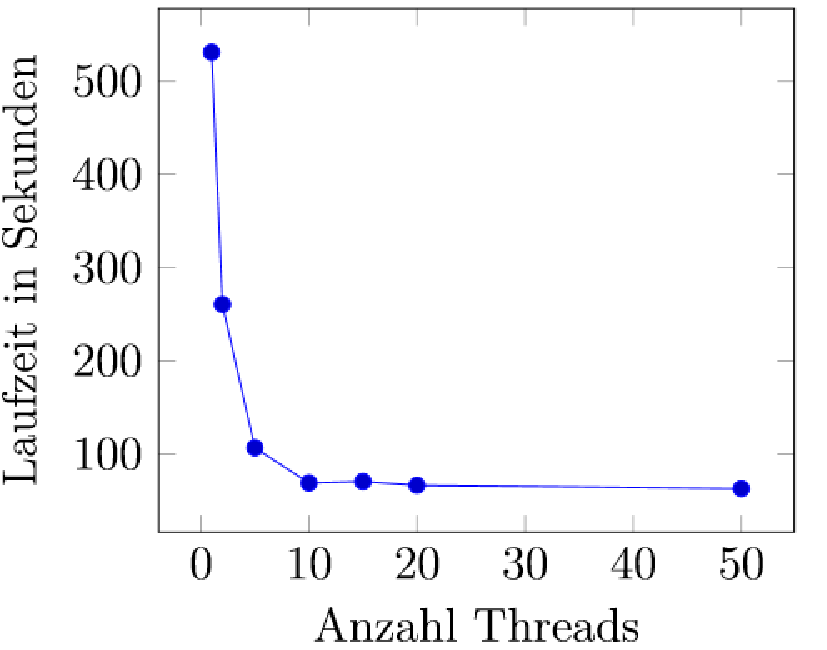
\includegraphics[scale=0.6]{images/laufzeiten}			 
		
	\end{minipage}
	\caption{Anzahl der Threads im Verhältnis zu Laufzeit}\label{fig.laufzeitListe}
\end{figure}

\listoffigures
\lstlistoflistings
\listoftables

% Quellenverzeichnis: ##############################################################################

% Für die Zitate verwende ich BiLaTeX mit Alphabetischem Stil (statt numeric)
% Das Quellen- oder Literaturverzeichnis ist in zwei separate Listen aufgeteilt:
% - Bücher
% - Sonstige Quellen
% Vor dem Einbinden, muss Biber auf die Thesis angewendet werden:
% $ biber thesis
% ACHTUNG: <thesis> OHNE DATEIENDUNG!
% Erst danach koennen die Zitate verwendet werden!!!!

\chapter*{Quellenverzeichnis}
\addcontentsline{toc}{chapter}{Quellenverzeichnis}
\printbibliography[type=book,heading=subbibliography,title={Bücher}]
\printbibliography[nottype=book,heading=subbibliography,title={Sonstige Quellen}]

\end{document}
